\documentclass[12pt,a4paper]{report}

% ---------- packages ----------
\usepackage[margin=1in]{geometry}
\usepackage{amsmath,amssymb}
\usepackage{graphicx}
\graphicspath{{../figures/}}
\usepackage{booktabs}
\usepackage{float}
\usepackage{xcolor}
\usepackage{listings}
\usepackage{caption}
\usepackage[hidelinks]{hyperref}
\usepackage{adjustbox}

%\lstset{
%  language=Python,
%  basicstyle=\ttfamily\small,
%  keywordstyle=\color{blue!60!black}\bfseries,
%  commentstyle=\color{green!40!black}\itshape,
%  stringstyle=\color{orange!70!black},
%  breaklines=true, frame=single, numbers=left, numberstyle=\tiny,
%  xleftmargin=2em, showstringspaces=false
%}

\lstdefinestyle{fancy}{
  backgroundcolor=\color{gray!10},
  basicstyle=\ttfamily,
  keywordstyle=\color{blue},
  commentstyle=\color{green!60!black},
  stringstyle=\color{red!70!black},
  frame=single,
  breaklines=true,
  showstringspaces=false
}

% ---------- front matter ----------
\title{\textbf{Topological and Structural Analysis of the Indian Stock Market}\\[0.6em]
\large A correlation network of Nifty 200 stocks from one year of daily prices}
\author{\textbf{Nikhil Kumar}\quad Roll Number: \textbf{\texttt{23205}}\\[0.3em]
ECS414/614 Network Science Theory and Applications\\ 2026-27-I}
\date{November 2026}

\begin{document}

\maketitle

\tableofcontents

% =====================================================================
\chapter{Introduction}

\section{Problem statement}
Stock prices are usually analysed one at a time, yet the stocks of a national market do not move independently. Firms in the same industry share suppliers, customers and regulation, and all stocks respond to common macroeconomic news. A useful way to represent this interdependence is a network in which each stock is a node and an edge records a strong co-movement between two stocks. Once the market is written as a graph, network science supplies tools for asking which stocks are central, whether the network breaks into sector-like groups, and how stable that structure is to the definition of ``strong'' co-movement.

\section{Objectives}
This project builds and analyses such a network for the constituents of the Nifty 200 index of the National Stock Exchange of India (NSE), using one year of daily adjusted closing prices. It asks four questions:
\begin{enumerate}
  \item Is the degree distribution random-like (exponential tail) or scale-free (power-law tail), so that a few stocks act as massive hubs?
  \item Which stocks are the most central by degree, betweenness and eigenvector measures, and do they agree with the major index heavyweights?
  \item Do triangles and clusters in the network stay within sectors, that is, is there sector homophily?
  \item How sensitive is the network's connectivity to the correlation threshold $r$?
\end{enumerate}

\section{Related work}
Mantegna \cite{mantegna1999} showed that a minimum spanning tree built from correlation-based distances between stocks groups firms by industry. Chi, Liu and Lau \cite{chi2010} study the stock market as a network built from return correlations. Moghadam et al.\ \cite{moghadam2019} apply centrality measures to the Iran stock market to identify influential stocks. This study follows the simpler threshold-based construction recommended in the course assignment, and extends it with a random-graph baseline, a random-matrix noise check and a permutation test for sector homophily.

\section{Organisation of the report}
Chapter 2 describes the data, cleaning and network construction. Chapter 3 visualises the network. Chapter 4 presents the four analyses (A to D). Chapter 5 interprets the results in economic terms and discusses limitations, and Chapter 6 concludes. Appendix A lists the key code functions. 

% =====================================================================
\chapter{Network Construction Methodology}

\section{Data source and scope}
The constituent list of Nifty 200 was obtained from the NSE Indices website \\(\texttt{ind\_Nifty200list.csv}). It contains 200 companies with their symbol and industry. Daily adjusted closing prices were downloaded with the \texttt{yfinance} Python package for the window 8 November 2025 to 8 November 2026, using \texttt{auto\_adjust=False} so that the \texttt{Adj Close} column is returned. Adjusted closes are used because they correct for splits and dividends, so the return series reflects total economic return. The raw downloads were cached locally, so the servers were queried only once. After cleaning, the sample covers 245 trading days, from 10 November 2025 to 6 November 2026, which gives $T=244$ daily return observations.

\section{Data cleaning}
Table~\ref{tab:data_quality} summarises the sample. A stock was dropped if more than 2\% of its trading days were missing. Three stocks failed this test, and all three are recent listings: ICICI Prudential AMC (first trade 19 December 2025, 11.7\% of days missing), Meesho (first trade 10 December 2025, 8.9\%) and VAML (first trade 15 June 2026, 59.1\%). Shorter gaps elsewhere were forward-filled for at most two days, and the remaining incomplete rows were removed so that all stocks share one trading calendar. Before cleaning, 0.427\% of all price cells were missing. The final sample is $N=197$ stocks.

\begin{table}
\centering
\caption{Data quality and sample construction.}
\label{tab:data_quality}
\begin{adjustbox}{max width=\textwidth}
\begin{tabular}{lr}
\toprule
 & value \\
\midrule
Requested tickers & 200.000 \\
Tickers returned with data & 200.000 \\
Kept after missing-data filter & 197.000 \\
Trading days after cleaning & 245.000 \\
Total missing cells before cleaning (\%) & 0.427 \\
\bottomrule
\end{tabular}
\end{adjustbox}
\end{table}


\section{Log returns}
For stock $i$ and day $t$, the daily logarithmic return is
\begin{equation} 
    R_i(t) = \ln\!\left(\frac{P_i(t)}{P_i(t-1)}\right) = \ln P_i(t) - \ln P_i(t-1),
\end{equation}
where $P_i(t)$ is the adjusted close. Log returns are additive over time and approximately symmetric, which makes them better suited to correlation analysis than raw prices, which trend and are not comparable across stocks.

\section{Pearson correlation matrix}
Over the $T=244$ return observations, the Pearson correlation between stocks $i$ and $j$ is
\begin{equation}
  \rho_{ij} = \frac{\sum_{t}\big(R_i(t)-\bar R_i\big)\big(R_j(t)-\bar R_j\big)}
  {\sqrt{\sum_{t}\big(R_i(t)-\bar R_i\big)^2}\,\sqrt{\sum_{t}\big(R_j(t)-\bar R_j\big)^2}},
\end{equation}
which gives a symmetric $197\times197$ matrix with unit diagonal. Across all $\binom{197}{2}=19{,}306$ stock pairs the mean correlation is $0.279$, the median is $0.274$, and the 90th percentile is $0.456$. The share of pairs above each threshold is $18.98\%$ for $\rho>0.4$, $5.73\%$ for $\rho>0.5$, $1.27\%$ for $\rho>0.6$, and $0.34\%$ for $\rho>0.7$.

\section{Edge definition: the unweighted threshold network}
Following the assignment, an unweighted adjacency matrix is built by connecting stocks $i$ and $j$ ($i\neq j$) if their correlation exceeds a threshold $r$:
\begin{equation}
  A_{ij} =
  \begin{cases}
    1, & \text{if } \rho_{ij} > r,\\
    0, & \text{otherwise.}
  \end{cases}
\end{equation}
The main analysis uses $r=0.6$, a value that keeps the network sparse enough to show structure while retaining 245 edges. Section~\ref{sec:threshold} shows how the results change across $r$. The network is undirected, since $\rho_{ij}=\rho_{ji}$.

Because a single threshold is a crude cut, a sampling-uncertainty check is useful. With $T=244$, the Fisher-$z$ 95\% interval for a correlation of $0.6$ is roughly $[0.51,\,0.67]$. Pairs whose correlation lies near $0.6$ may therefore enter or leave the network under a different sample window. This is the reason the threshold study matters for interpretation.

\section{Checks and caveats}
Three checks were performed in the notebook. The matrix is symmetric with unit diagonal. The log-return formula agrees with the difference of log prices. The handshake lemma $\sum_i k_i = 2M$ holds for the network.

Two caveats matter for interpretation. The first is noise. With $N/T = 197/244 = 0.807$, the Marchenko--Pastur upper bound for pure-noise eigenvalues is $\lambda_+=(1+\sqrt{N/T})^2 = 3.604$. Five eigenvalues of the correlation matrix lie above this bound, so they carry genuine common structure, while the rest are consistent with noise. The second is the market mode. The largest eigenvalue is $\lambda_1 = 60.21$, roughly 17 times the noise bound, and the average pairwise correlation of $0.279$ is well above zero. A large common factor inflates correlations across the board, so the threshold network partly reflects the market rather than purely sector-level structure. Chapter 5 returns to this.

\section{Code}
The functions used to build the network and compute the homophily statistics are listed in Appendix A.

However, the complete pipeline is in the accompanying notebook \\\texttt{Topological\_Analysis\_Nifty200.ipynb}, which can be found at this Google drive link: \href{https://drive.google.com/file/d/18AM20b_h5e0STOYt2iY9u7jkNsMmPmtY/view?usp=sharing}{[click here]}.

% =====================================================================
\chapter{Visualising the Network}

Figure~\ref{fig:network} shows the giant connected component of the network at $r=0.6$. The component has 69 stocks and 35\% of the sample. Isolated stocks are removed for readability. Node colour encodes the sector, node size encodes degree, and the ten highest-degree stocks are labelled. The layout is a force-directed spring embedding, so nodes that share many links are drawn close together. 

\begin{figure}[H]
\centering
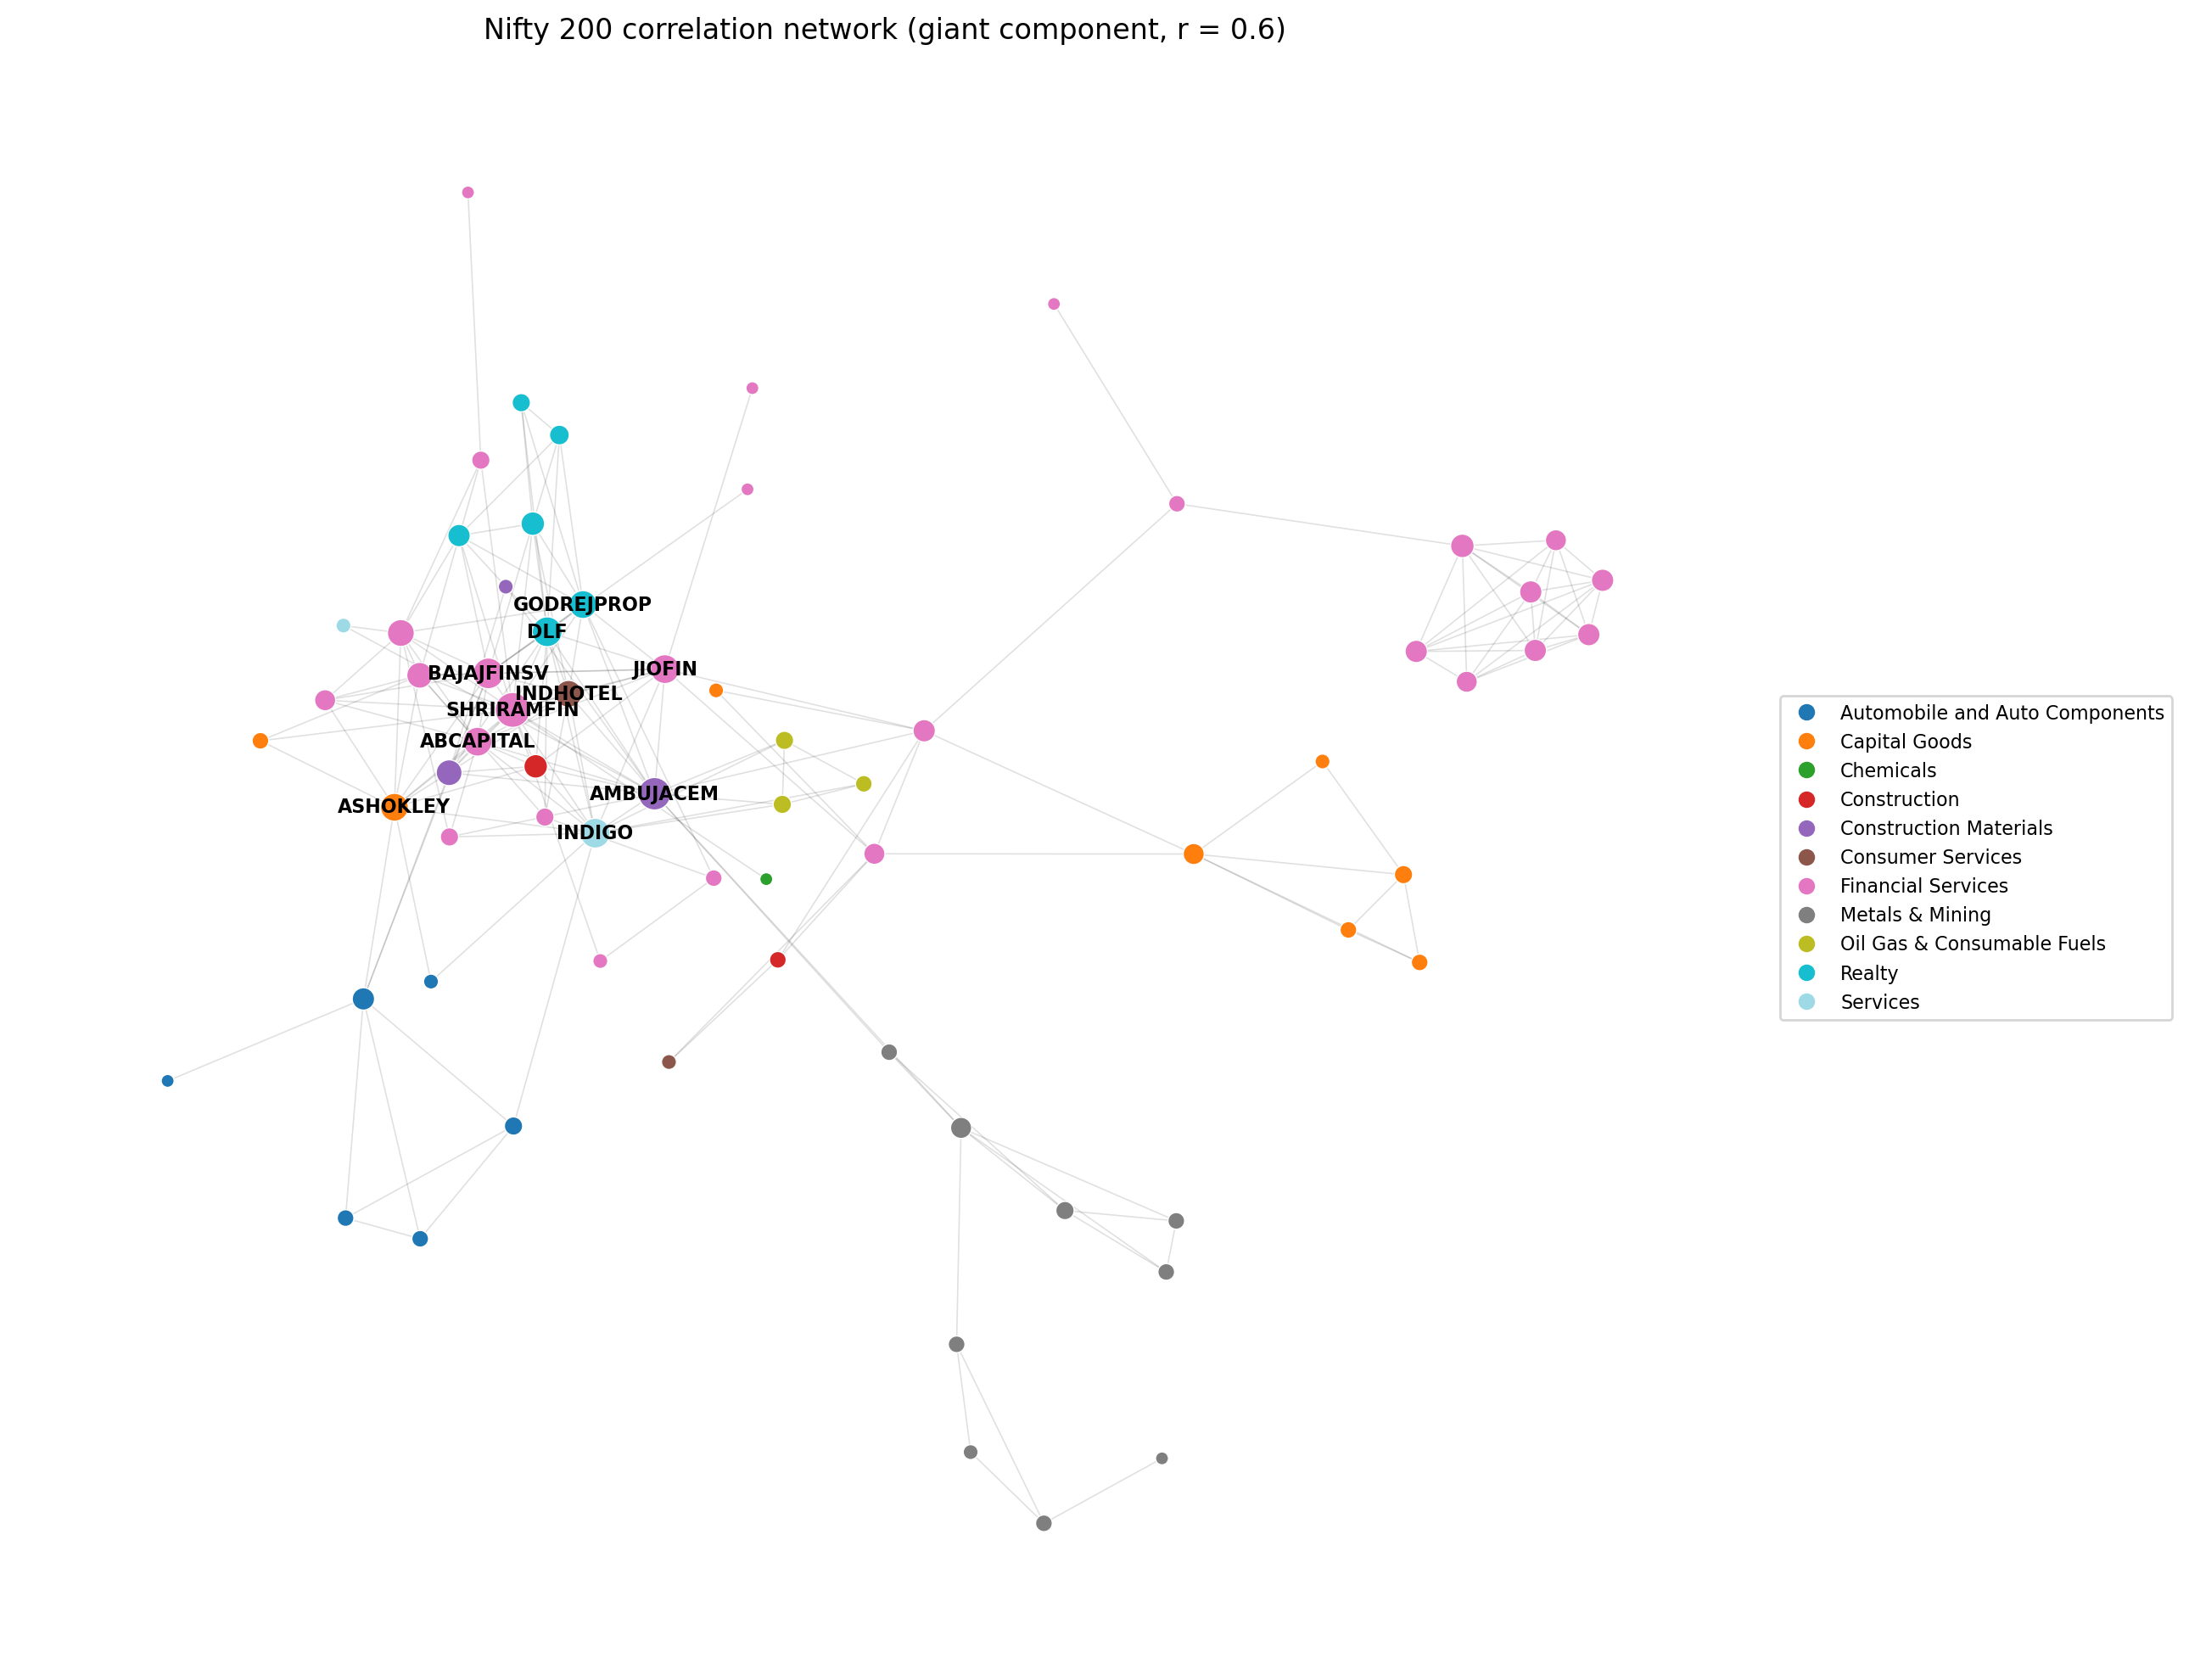
\includegraphics[width=\linewidth]{network_giant_component.png}
\caption{Giant component of the Nifty 200 correlation network at $r=0.6$. Colour = sector; size = degree.}
\label{fig:network}
\end{figure}

The figure shows three features. First, the component is not one undifferentiated cloud. Financial Services stocks (pink) form a dense, distinct group at the top left and a second group in the centre, and Metals \& Mining (grey) forms a separate branch at the top right. Second, the dense core is a mix of sectors: Financial Services, Realty (cyan), Consumer Services (brown), Capital Goods (orange) and Automobiles (blue) meet around the highest-degree stocks SHRIRAMFIN, DLF, GODREJPROP, BAJAJFINSV and INDHOTEL. This mixing foreshadows the homophily result in Section~\ref{sec:homophily}. Third, a few stocks sit on long chains between groups, such as AMBUJACEM, which appears to link the financial core with the cement and Oil \& Gas stocks. These bridging nodes reappear in the betweenness analysis.

% =====================================================================
\chapter{Analyses of Network Parameters}

Table~\ref{tab:graph_summary} gives the basic properties of the network at $r=0.6$.

\begin{table}
\centering
\caption{Basic properties of the unweighted network.}
\label{tab:graph_summary}
\begin{adjustbox}{max width=\textwidth}
\begin{tabular}{lr}
\toprule
 & value \\
\midrule
Nodes N & 197.0000 \\
Edges M & 245.0000 \\
Density & 0.0127 \\
Average degree & 2.4873 \\
Isolated nodes & 92.0000 \\
Connected components & 105.0000 \\
Giant component size & 69.0000 \\
Giant component fraction & 0.3503 \\
\bottomrule
\end{tabular}
\end{adjustbox}
\end{table}


The network is very sparse. Its density is $0.0127$ and its average degree is $2.49$. Ninety-two of the 197 stocks (46.7\%) have no neighbour at all, and the network splits into 105 components. The largest component contains 69 stocks. Every statistic in this chapter that refers to connectivity must be read with that in mind. 

\section{Degree Distribution Plot and Interpretation}
\label{sec:degree}

Figure~\ref{fig:degree} shows the degree distribution on a linear scale, on a log-log scale, and as the complementary cumulative distribution $P(K\ge k)$. The CCDF is used for the tail tests because it is less noisy than the histogram. An exponential tail appears as a straight line on a semi-log plot, whereas a power-law tail appears as a straight line on log-log axes.

\begin{figure}[H]
\centering
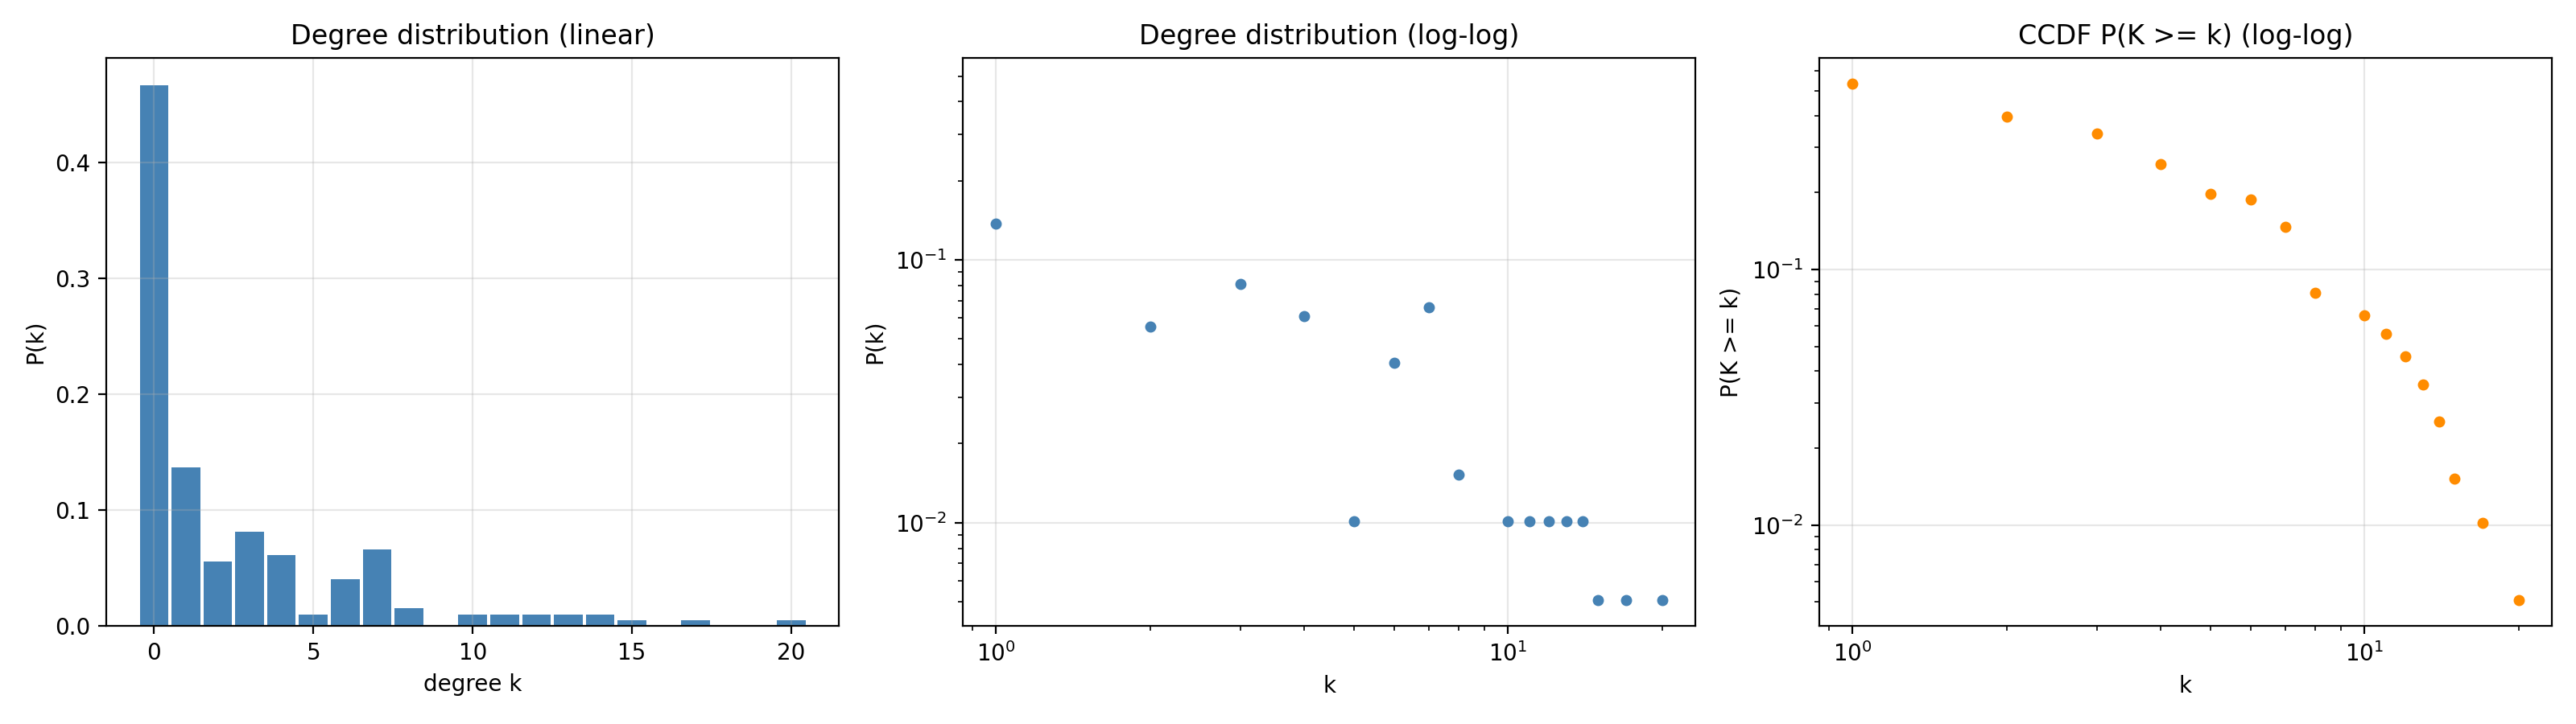
\includegraphics[width=\linewidth]{degree_distribution.png}
\caption{Degree distribution: linear histogram, log-log histogram $P(k)$, and log-log CCDF.}
\label{fig:degree}
\end{figure}

Table~\ref{tab:degree_fit} compares the two fits on the tail $k\ge3$, which contains 67 stocks and 14 distinct CCDF points. The exponential fit is a straight line of $\ln P(K\ge k)$ against $k$; the power-law fit is a straight line of $\ln P(K\ge k)$ against $\ln k$. The exponent $\alpha$ is estimated by the maximum-likelihood approximation for discrete data.

\begin{table}
\centering
\caption{Degree distribution summary and tail-fit comparison.}
\label{tab:degree_fit}
\begin{adjustbox}{max width=\textwidth}
\begin{tabular}{lr}
\toprule
 & value \\
\midrule
Mean degree & 2.487 \\
Max degree & 20.000 \\
R-squared, exponential fit (semi-log CCDF) & 0.989 \\
R-squared, power-law fit (log-log CCDF) & 0.909 \\
Power-law exponent alpha (MLE, tail k from 3) & 2.213 \\
\bottomrule
\end{tabular}
\end{adjustbox}
\end{table}


The degree distribution is strongly skewed: 47\% of stocks are isolated, the mean degree is 2.5, and the largest degree is 20, held by SHRIRAMFIN. On the tail, the exponential fit is clearly better, with $R^2=0.989$ against $0.909$ for the power law. The estimated power-law exponent, $\alpha=2.21$, lies in the range usually seen for scale-free networks, but the evidence for a power law is weak, for three reasons. The tail is short, with only 14 CCDF points. The power-law fit has a visible bend at intermediate degrees (Figure~\ref{fig:degree}, right). And the sample has only 197 nodes, so the maximum degree is limited by construction. The fair conclusion is that the network is not clearly scale-free. Its tail decays roughly exponentially, with no single extreme hub that dominates the structure. The hubs that do exist, SHRIRAMFIN (degree 20), AMBUJACEM (17) and BAJAJFINSV (15), are moderately connected rather than dominant. 

\section{The Top-10 Centrality Leaderboard}

Three centrality measures were computed. Degree centrality counts the peers a stock moves with. Betweenness centrality measures how often a stock lies on shortest paths between other stocks, so it identifies bridges between groups. Eigenvector centrality gives a high score to stocks linked to other well-connected stocks. Tables~\ref{tab:top10_degree}, \ref{tab:top10_betweenness} and \ref{tab:top10_eigenvector} list the top ten for each measure.

\begin{table}
\centering
\caption{Top-10 stocks by degree centrality.}
\label{tab:top10_degree}
\begin{adjustbox}{max width=\textwidth}
\begin{tabular}{lllr}
\toprule
 & Company & Sector & Degree C \\
\midrule
SHRIRAMFIN.NS & Shriram Finance Ltd. & Financial Services & 0.1020 \\
AMBUJACEM.NS & Ambuja Cements Ltd. & Construction Materials & 0.0867 \\
BAJAJFINSV.NS & Bajaj Finserv Ltd. & Financial Services & 0.0765 \\
INDIGO.NS & InterGlobe Aviation Ltd. & Services & 0.0714 \\
DLF.NS & DLF Ltd. & Realty & 0.0714 \\
ABCAPITAL.NS & Aditya Birla Capital Ltd. & Financial Services & 0.0663 \\
JIOFIN.NS & Jio Financial Services Ltd. & Financial Services & 0.0663 \\
GODREJPROP.NS & Godrej Properties Ltd. & Realty & 0.0612 \\
ASHOKLEY.NS & Ashok Leyland Ltd. & Capital Goods & 0.0612 \\
INDHOTEL.NS & Indian Hotels Co. Ltd. & Consumer Services & 0.0561 \\
\bottomrule
\end{tabular}
\end{adjustbox}
\end{table}

\begin{table}
\centering
\caption{Top-10 stocks by betweenness centrality.}
\label{tab:top10_betweenness}
\begin{adjustbox}{max width=\textwidth}
\begin{tabular}{lllr}
\toprule
 & Company & Sector & Betweenness C \\
\midrule
AMBUJACEM.NS & Ambuja Cements Ltd. & Construction Materials & 0.0490 \\
IREDA.NS & Indian Renewable Energy Development Agency Ltd. & Financial Services & 0.0450 \\
RECLTD.NS & REC Ltd. & Financial Services & 0.0282 \\
JIOFIN.NS & Jio Financial Services Ltd. & Financial Services & 0.0265 \\
PNB.NS & Punjab National Bank & Financial Services & 0.0224 \\
TATASTEEL.NS & Tata Steel Ltd. & Metals \& Mining & 0.0213 \\
SHRIRAMFIN.NS & Shriram Finance Ltd. & Financial Services & 0.0172 \\
MAZDOCK.NS & Mazagoan Dock Shipbuilders Ltd. & Capital Goods & 0.0134 \\
INDIGO.NS & InterGlobe Aviation Ltd. & Services & 0.0123 \\
HINDALCO.NS & Hindalco Industries Ltd. & Metals \& Mining & 0.0102 \\
\bottomrule
\end{tabular}
\end{adjustbox}
\end{table}

\begin{table}
\centering
\caption{Top-10 stocks by eigenvector centrality.}
\label{tab:top10_eigenvector}
\begin{adjustbox}{max width=\textwidth}
\begin{tabular}{lllr}
\toprule
 & Company & Sector & Eigenvector C \\
\midrule
SHRIRAMFIN.NS & Shriram Finance Ltd. & Financial Services & 0.3579 \\
BAJAJFINSV.NS & Bajaj Finserv Ltd. & Financial Services & 0.2883 \\
ABCAPITAL.NS & Aditya Birla Capital Ltd. & Financial Services & 0.2762 \\
DLF.NS & DLF Ltd. & Realty & 0.2693 \\
AMBUJACEM.NS & Ambuja Cements Ltd. & Construction Materials & 0.2560 \\
JIOFIN.NS & Jio Financial Services Ltd. & Financial Services & 0.2536 \\
INDHOTEL.NS & Indian Hotels Co. Ltd. & Consumer Services & 0.2492 \\
INDIGO.NS & InterGlobe Aviation Ltd. & Services & 0.2284 \\
GODREJPROP.NS & Godrej Properties Ltd. & Realty & 0.2272 \\
ASHOKLEY.NS & Ashok Leyland Ltd. & Capital Goods & 0.2186 \\
\bottomrule
\end{tabular}
\end{adjustbox}
\end{table}


Table~\ref{tab:centrality_corr} gives the Spearman rank correlation between the three measures.
Table~\ref{tab:heavyweights} gives the ranks of eight major index heavyweights. A rank of 106 means the stock is isolated at $r=0.6$, since 106 is the shared rank of all 105 non-zero-degree tied nodes.

\begin{table}
\centering
\caption{Spearman rank correlation between centrality measures.}
\label{tab:centrality_corr}
\begin{adjustbox}{max width=\textwidth}
\begin{tabular}{lrrr}
\toprule
 & degree & betweenness & eigenvector \\
\midrule
degree & 1.000 & 0.790 & 0.941 \\
betweenness & 0.790 & 1.000 & 0.719 \\
eigenvector & 0.941 & 0.719 & 1.000 \\
\bottomrule
\end{tabular}
\end{adjustbox}
\end{table}

\begin{table}
\centering
\caption{Centrality ranks of major index heavyweights.}
\label{tab:heavyweights}
\begin{adjustbox}{max width=\textwidth}
\begin{tabular}{lrrr}
\toprule
 & degree & betweenness & eigenvector \\
\midrule
RELIANCE.NS & 106 & 58 & 106 \\
TCS.NS & 17 & 35 & 73 \\
HDFCBANK.NS & 106 & 58 & 106 \\
ICICIBANK.NS & 106 & 58 & 106 \\
INFY.NS & 17 & 35 & 73 \\
BHARTIARTL.NS & 106 & 58 & 106 \\
ITC.NS & 106 & 58 & 106 \\
SBIN.NS & 30 & 58 & 67 \\
\bottomrule
\end{tabular}
\end{adjustbox}
\end{table}


\subsection*{Degree and eigenvector agree}
The Spearman correlation between degree and eigenvector centrality is $0.941$, so the two measures pick almost the same stocks. Degree and betweenness agree less closely ($0.790$), and eigenvector and betweenness agree least ($0.719$). The gap shows that betweenness is measuring something different. A stock can be well connected without lying between groups, and vice versa.

\subsection*{Who is central}
The degree and eigenvector leaders are dominated by the Financial Services group: SHRIRAMFIN, BAJAJFINSV, ABCAPITAL and JIOFIN all appear in the top ten by degree or eigenvector. Financial Services is the largest sector in the sample, with 47 stocks, so this result partly reflects size. Many financial stocks have several peers above the threshold. Realty, Capital Goods and Services names (DLF, GODREJPROP, ASHOKLEY, INDIGO) also rank highly, which fits the dense Realty cluster found in Section~\ref{sec:homophily}. 

The betweenness leaders tell a different story. AMBUJACEM, which has the highest betweenness, is a cement company, yet it sits at the centre of the network's shortest paths. It appears to bridge the financial core and the construction and energy stocks. IREDA and RECLTD are the two power-sector lenders. Their high betweenness links the financial group to the power and energy stocks, which is economically plausible: power-sector finance is exposed both to lending markets and to the power cycle. PNB and TATASTEEL (metals) also bridge groups. These bridging stocks are where a shock in one sector would most likely pass into another.

\subsection*{Index heavyweights}
Table~\ref{tab:heavyweights} shows that network centrality does not track index weight. RELIANCE, HDFCBANK, ICICIBANK, ITC and BHARTIARTL are isolated at $r=0.6$, even though they are among the largest companies. The reason is visible in their nearest neighbours. The highest correlation of RELIANCE with any other stock is $0.495$ (JIOFIN), of ITC is $0.540$, and of BHARTIARTL is $0.368$. Reliance is a conglomerate spanning oil, telecom and retail, so no single peer group drives its returns. Bharti Airtel's strongest peer is ITC, at only $0.368$, and its other telecom peers in the sample (Vodafone Idea, Tata Communications and Indus Towers) are no more closely correlated with it. The two banks are closer to the threshold. HDFCBANK's strongest peer is AXISBANK at $0.570$, and ICICIBANK's is AXISBANK at $0.594$. Both lie within the sampling interval of the $0.6$ threshold, so the banks would enter the network at a slightly lower $r$. 
Their isolation is therefore a threshold effect rather than evidence that they are unrelated to banking.

TCS and INFY sit at the centre of the Information Technology cluster, with a correlation of $0.779$ between them, the strongest pair in the sample. They are the most tightly coupled pair in the market. SBIN ranks 30th by degree and 58th by betweenness, with its strongest link to PNB at $0.635$.

\section{Local Clustering Coefficient and Sector Homophily}
\label{sec:homophily}

The average clustering coefficient is $0.268$, against $0.0094\pm0.0069$ for 200 random graphs $G(n,m)$ with the same 197 nodes and 245 edges. Transitivity, the fraction of connected triples that close into triangles, is $0.536$. Clustering is therefore about 28 times the random baseline. In practical terms, when stock A correlates strongly with stock B and B with C, A and C are very likely to correlate strongly as well. The network has 309 triangles, and 155 of them (50.2\%) have all three stocks in the same sector.

Sector homophily is measured in two ways. The homophily ratio is the observed share of within-sector edges divided by the expected share $\sum_s p_s^2$ under random mixing, where $p_s$ is the fraction of stocks in sector $s$. The permutation test shuffles sector labels 2,000 times and records how often a random labelling produces a within-sector share at least as large as the observed one.

\begin{itemize}
  \item Observed within-sector edge share: $0.633$.
  \item Expected under random mixing: $0.105$.
  \item Homophily ratio: $6.02$.
  \item Permutation test: the null mean is $0.100$ and the 95th percentile is $0.143$. The observed value exceeds every one of the 2,000 shuffles, so $p<0.001$ (the smallest value the test can report with 2,000 permutations is $1/2001\approx0.0005$).
\end{itemize}

Edges are therefore strongly concentrated within sectors. A correlation that survives a threshold of 0.6 is much more likely to join two stocks from the same industry than chance would allow. The average correlation inside sectors is $0.402$, against $0.265$ across sectors, which confirms the pattern at the level of the full correlation matrix.

Table~\ref{tab:sector_homophily} shows that homophily is uneven across sectors.

\begin{table}
\centering
\caption{Within-sector structure of the network.}
\label{tab:sector_homophily}
\begin{adjustbox}{max width=\textwidth}
\begin{tabular}{lrrrr}
\toprule
 & stocks & internal edges & internal density & within-sector share of endpoints \\
\midrule
Financial Services & 47 & 66 & 0.061 & 0.717 \\
Capital Goods & 24 & 15 & 0.054 & 0.638 \\
Healthcare & 15 & 0 & 0.000 & -- \\
Automobile and Auto Components & 14 & 7 & 0.077 & 0.700 \\
Fast Moving Consumer Goods & 14 & 1 & 0.011 & 1.000 \\
Metals \& Mining & 11 & 13 & 0.236 & 0.812 \\
Consumer Services & 11 & 0 & 0.000 & 0.000 \\
Information Technology & 10 & 27 & 0.600 & 1.000 \\
Oil Gas \& Consumable Fuels & 9 & 4 & 0.111 & 0.615 \\
Power & 9 & 4 & 0.111 & 0.615 \\
Consumer Durables & 8 & 1 & 0.036 & 1.000 \\
Realty & 6 & 14 & 0.933 & 0.560 \\
Chemicals & 5 & 0 & 0.000 & 0.000 \\
Services & 4 & 0 & 0.000 & 0.000 \\
Telecommunication & 4 & 0 & 0.000 & -- \\
Construction Materials & 3 & 3 & 1.000 & 0.207 \\
Construction & 2 & 0 & 0.000 & 0.000 \\
Textiles & 1 & 0 & -- & -- \\
\bottomrule
\end{tabular}
\end{adjustbox}
\end{table}


Three patterns stand out. Realty (density $0.93$ of six stocks) and Information Technology (density $0.60$ of ten stocks) are almost fully internally connected, so these are the clearest industry clusters. Metals \& Mining (density $0.24$) and Financial Services (density $0.06$ across 47 stocks) are internally connected too, though less tightly. Financial Services is large, so its low density still produces 66 internal edges. In contrast, Healthcare (15 stocks), Consumer Services (11), and Chemicals (5) have no internal edges at all. Pharmaceutical stocks, in particular, co-move with the broad market and with each other less strongly than their sector label suggests. Construction Materials has full internal density across its three stocks, but only 21\% of its edge endpoints stay inside the sector, because its links run out to other groups.

\section{Threshold Sensitivity Analysis}
\label{sec:threshold}

The network was rebuilt for $r\in\{0.30,0.35,\dots,0.85\}$. Table~\ref{tab:threshold} and Figure~\ref{fig:sens} show how edges, connectivity, average path length inside the giant component, clustering and the homophily ratio change with $r$. The average path length is computed only inside the giant component, because the full graph is disconnected at most thresholds.

{\small\begin{table}
\centering
\caption{Threshold sensitivity of network structure.}
\label{tab:threshold}
\begin{adjustbox}{max width=\textwidth}
\begin{tabular}{lrrrrrrrrr}
\toprule
 & edges & density & isolated & components & giant size & giant fraction & avg path (giant) & avg clustering & homophily ratio \\
\midrule
0.30 & 8219 & 0.426 & 0 & 1 & 197 & 1.000 & 1.673 & 0.786 & 1.723 \\
0.35 & 5760 & 0.298 & 1 & 3 & 194 & 0.985 & 1.929 & 0.734 & 2.051 \\
0.40 & 3664 & 0.190 & 9 & 12 & 184 & 0.934 & 2.342 & 0.633 & 2.440 \\
0.45 & 2056 & 0.106 & 23 & 30 & 152 & 0.772 & 2.275 & 0.573 & 3.000 \\
0.50 & 1107 & 0.057 & 41 & 52 & 126 & 0.640 & 2.499 & 0.414 & 3.560 \\
0.55 & 514 & 0.027 & 72 & 83 & 91 & 0.462 & 2.640 & 0.340 & 4.685 \\
0.60 & 245 & 0.013 & 92 & 105 & 69 & 0.350 & 3.579 & 0.268 & 6.022 \\
0.65 & 113 & 0.006 & 119 & 138 & 11 & 0.056 & 2.218 & 0.206 & 8.003 \\
0.70 & 66 & 0.003 & 143 & 158 & 8 & 0.041 & 1.786 & 0.154 & 8.509 \\
0.75 & 27 & 0.001 & 164 & 176 & 6 & 0.030 & 1.400 & 0.051 & 8.461 \\
0.80 & 8 & 0.000 & 184 & 190 & 3 & 0.015 & 1.000 & 0.015 & 8.329 \\
0.85 & 2 & 0.000 & 194 & 195 & 3 & 0.015 & 1.333 & 0.000 & 9.519 \\
\bottomrule
\end{tabular}
\end{adjustbox}
\end{table}
}

\begin{figure}[H]
\centering
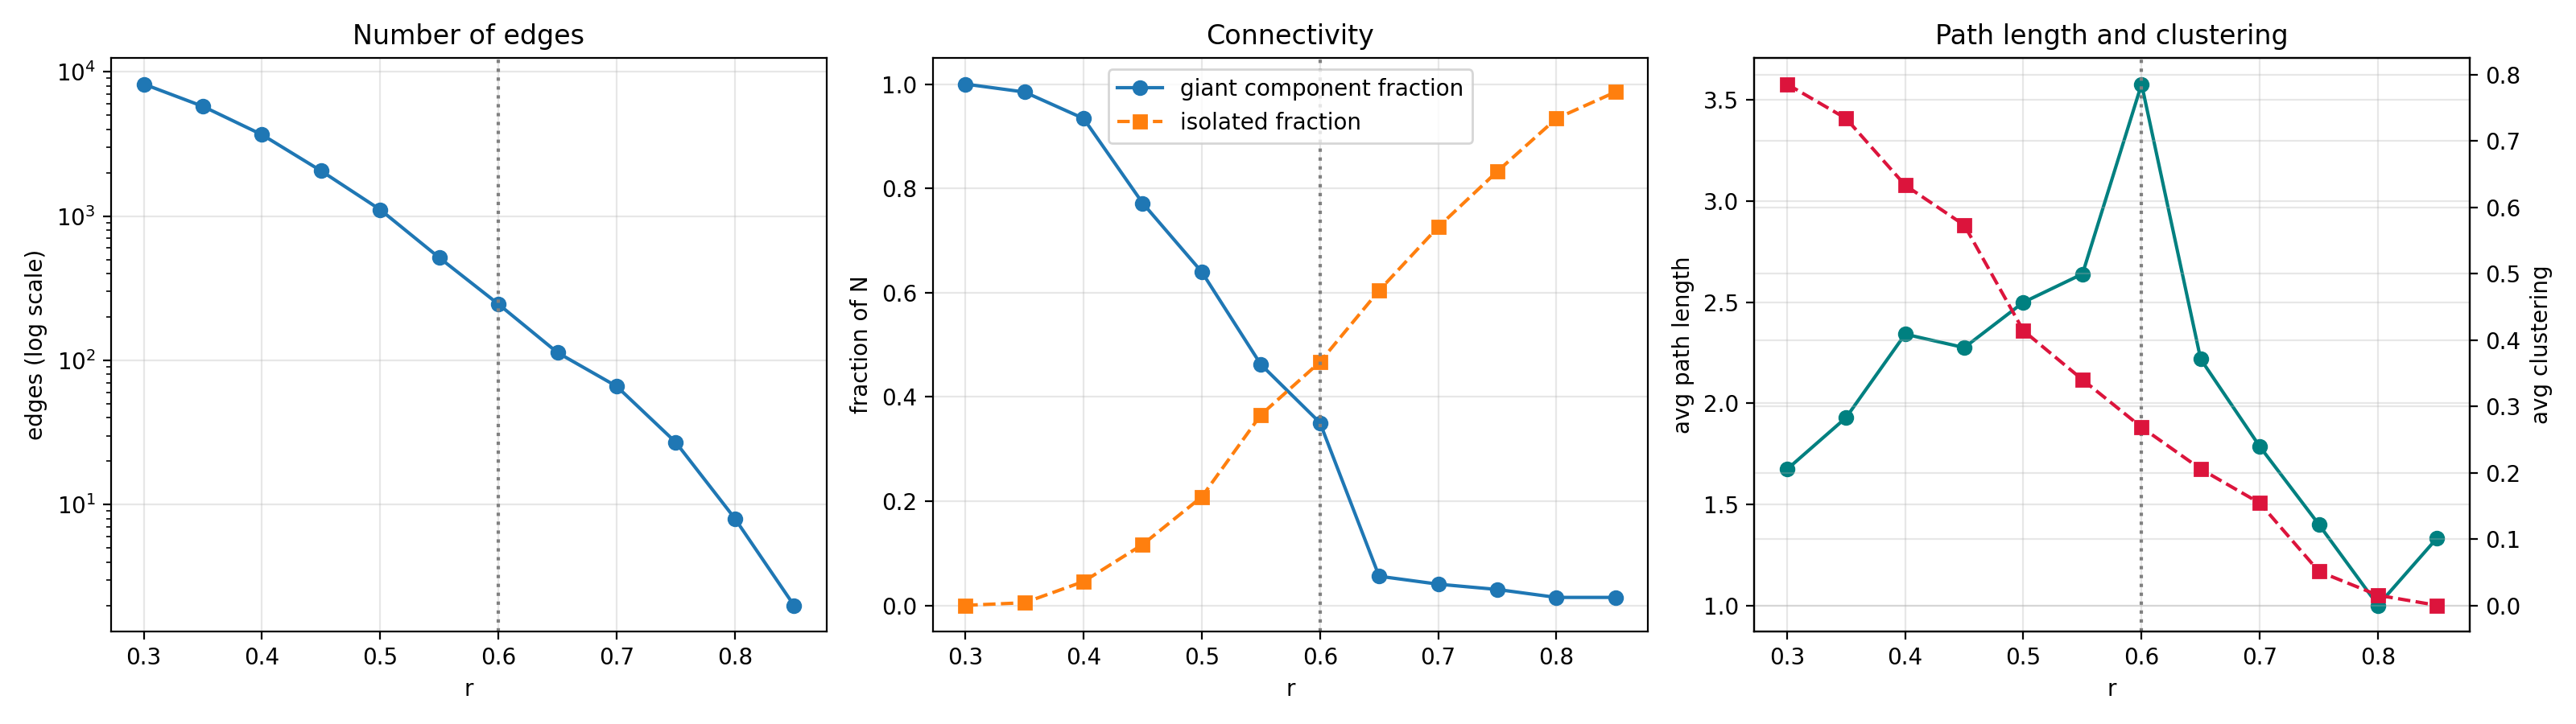
\includegraphics[width=\linewidth]{threshold_sensitivity.png}
\caption{Effect of the correlation threshold $r$ on edges, connectivity, path length and clustering.}
\label{fig:sens}
\end{figure}

The number of edges falls steeply, from 8,219 at $r=0.30$ to 514 at $r=0.55$, to 245 at $r=0.60$, and to two at $r=0.85$. Connectivity has a clear breaking point. The giant component contains 98.5\% of stocks at $r=0.35$, 64\% at $r=0.50$, and 35\% at $r=0.60$. Above $r=0.65$ it falls to 11 stocks, which is no longer a network-scale structure. The network is therefore robust to a loose definition of a connection but fragile to a strict one. The threshold at which it breaks apart lies between $0.55$ and $0.65$.

Clustering declines steadily, from $0.786$ at $r=0.30$ to $0.268$ at $r=0.60$. The homophily ratio rises steadily in the opposite direction, from $1.72$ to about $8.5$ at $r=0.70$. This is the most informative pattern in the sensitivity study. The strongest co-movements are the ones that stay inside sectors, and the weaker links that connect sectors disappear first. So a stricter threshold yields a network that looks more like its sector structure, though a smaller and more fragmented one.

The average path length inside the giant component ranges between about 1.0 and 3.6 across thresholds, but it is not comparable across rows. At $r=0.60$ the giant component has only 69 nodes, while at $r=0.30$ it has all 197, so the path values describe different-sized graphs. The apparent rise at $r=0.60$ should not be read as the network becoming less cohesive. The fair statement is that path length is short wherever the giant component is large.

The main analysis uses $r=0.6$, the value chosen before this sensitivity study was run. It keeps the network sparse while retaining 245 edges, but its giant component is small. On the evidence of Table~\ref{tab:threshold}, a more robust choice would be $r=0.50$, which keeps 64\% of stocks in one component and has a homophily ratio of 3.56. The results in Chapters 4 and 5 should be read as describing the strongest co-movements, and the $r=0.50$ row of Table~\ref{tab:threshold} gives the comparison.

% =====================================================================
\chapter{Interpretation and Discussion}

Taken together, the results describe a market whose co-movements are strongly organised by industry, with a small number of bridging stocks and a common market factor running beneath them. 

\textbf{Structure is sectoral, not scale-free.} The degree distribution is skewed, with almost half the stocks unconnected and a short tail. The exponential form fits better than a power law, so no single stock dominates the network as a systemic hub. The most connected stocks are moderately connected, not dominant. Systemic risk in this sample is better described as a set of sector-level channels than as a single hub that could topple the market.

\textbf{Centrality points to finance and to bridges.} Degree and eigenvector centrality both point to Financial Services, partly because it is the largest sector. Betweenness points to a different set of stocks: the cement, power-finance and metals names that connect the financial core to the infrastructure and energy economy. For portfolio purposes, a holding in AMBUJACEM, IREDA or RECLTD adds exposure to several clusters at once, which makes it less diversifying than its sector label suggests. A holding in a financial stock adds exposure to a large, tightly connected group, so diversification within finance is limited.

\textbf{Index weight is not network centrality.} Several large companies (Reliance, both private banks, ITC and Bharti Airtel) have no neighbour above $r=0.6$. Their returns are driven either by a diversified business mix or by factors that the correlation network does not capture in one year. Market capitalisation and network position are different things, and the network adds information that index weight does not show.

\textbf{Sector homophily is real, and it is strongest where it is expected.} The homophily ratio of 6.0 and the permutation result leave little doubt that correlations concentrate inside sectors. The clearest clusters are Realty and Information Technology. The absence of internal links in Healthcare and Consumer Services is more surprising, and it suggests that for these sectors the sector label is a weak guide to co-movement in this window.

\textbf{The market mode and the threshold are the main caveats.} The largest eigenvalue, 60.2, is far above the noise bound of 3.6, so a common factor drives much of the correlation. Some of the sector clustering may therefore reflect the market factor combined with sector sensitivity to it, not purely industry-specific linkages. A useful next step would be to remove the market factor (for example, by using residuals from a regression on an index) and check whether the sector structure survives. The threshold also matters. Because HDFCBANK and ICICIBANK are just below $0.6$, a slightly looser threshold would connect them, and the qualitative conclusion that banks are not central would change.

\subsection*{Limitations}
\begin{itemize}
  \item \textbf{One window, one threshold.} One year of data reflects a particular market regime. Results may differ in other years, and the sample of 244 returns gives correlations an uncertainty of about $\pm0.08$ at $\rho=0.6$.
  \item \textbf{Linear dependence only.} Pearson correlation misses nonlinear and tail dependence, which matter most in crises.
  \item \textbf{Market mode.} A dominant common factor inflates correlations across the board. Removing it, for example with market-model residuals, would reveal finer structure.
  \item \textbf{Noise.} With $N/T=0.807$, much of the correlation matrix is consistent with noise. Only five eigenvalues exceed the Marchenko--Pastur bound.
  \item \textbf{Survivorship bias.} The constituent list is the current index membership, not the membership at the start of the window. Three recent listings were excluded for lack of data.
  \item \textbf{Null model.} The homophily baseline assumes random mixing with respect to sector sizes. It does not control for degree, so part of the excess within-sector edges may come from high-degree financial stocks.
  \item \textbf{Correlation is not causation.} A link indicates co-movement, not that one firm drives another.
\end{itemize}

% =====================================================================
\chapter{Conclusion}

Using one year of daily adjusted prices for 197 Nifty 200 stocks, this study built an unweighted correlation network at $r=0.6$ and found a sparse, sector-organised structure. Almost half the stocks have no strong peer, and the network's tail decays roughly exponentially rather than as a power law, so it has no single dominant hub. The most central stocks by degree and eigenvector come mostly from Financial Services, while betweenness highlights bridging stocks in cement, power finance and metals. Co-movement is strongly sector-homophilous, with a within-sector edge share six times the random expectation, and the clearest clusters are Realty and Information Technology. Index heavyweights such as Reliance and the two large private banks are isolated at this threshold, which shows that network position and index weight are different measures.

The network is robust to a loose definition of a connection and fragile to a strict one. The giant component falls from 64\% of stocks at $r=0.5$ to 35\% at $r=0.6$. The most useful next step is to remove the common market factor and test whether the sector structure survives, which would show how much of the clustering is industry-specific rather than market-driven.

% =====================================================================
\begin{thebibliography}{9}
\bibitem{chi2010}
Chi, K. Tse, Jing Liu and Francis C.M.\ Lau.
\newblock A network perspective of the stock market.
\newblock \emph{Journal of Empirical Finance}, 17(4):659--667, 2010.

\bibitem{moghadam2019}
Moghadam, Hadi Esmaeilpour, et al.
\newblock Complex networks analysis in Iran stock market: The application of centrality.
\newblock \emph{Physica A: Statistical Mechanics and its Applications}, 531:121800, 2019.

\bibitem{mantegna1999}
Mantegna, Rosario N.
\newblock Hierarchical structure in financial markets.
\newblock \emph{The European Physical Journal B}, 11(1):193--197, 1999.
\end{thebibliography}

% =====================================================================
\appendix
\chapter{Notebook Code}
The complete code of the analysis notebook \texttt{Analysis of Stocks in NSE.ipynb} is reproduced below, cell by cell in execution order. Markdown cells and outputs are omitted. Cells are numbered 1 to 29 in the order they run.

\subsection*{Code cell 1}
\begin{lstlisting}[style=fancy]
import os, time, json, warnings
import numpy as np
import pandas as pd
import networkx as nx
import matplotlib.pyplot as plt
import requests
import yfinance as yf
from scipy import stats
\end{lstlisting}

\subsection*{Code cell 2}
\begin{lstlisting}[style=fancy]
warnings.filterwarnings("ignore", category=FutureWarning)
np.random.seed(42)
plt.rcParams.update({"figure.dpi": 110, "axes.grid": True, "grid.alpha": 0.3})
\end{lstlisting}

\subsection*{Code cell 3}
\begin{lstlisting}[style=fancy]
URL = "https://www.niftyindices.com/IndexConstituent/ind_nifty200list.csv"
DATA_DIR, FIG_DIR, TAB_DIR = "data", "figures", "tables"
for d in (DATA_DIR, FIG_DIR, TAB_DIR):
    os.makedirs(d, exist_ok=True)
\end{lstlisting}

\subsection*{Code cell 4}
\begin{lstlisting}[style=fancy]
start, end = "2025-11-08", "2026-11-08"  # 1 yr daily data
r_main = 0.6  # main correlation threshold r
max_missing = 0.02  # to drop a stock if more than 2% of dayas are missing
k_min = 3  # lower cut-off for the power law comparision
\end{lstlisting}

\subsection*{Code cell 5}
\begin{lstlisting}[style=fancy]
FILE = f"{DATA_DIR}/nifty200list.csv"

if not os.path.exists(FILE):
    resp = requests.get(URL, headers={"User-Agent": "Mozilla/5.0"}, timeout=30)
    resp.raise_for_status()
    with open(FILE, "w") as f:
        f.write(resp.text)
\end{lstlisting}

\subsection*{Code cell 6}
\begin{lstlisting}[style=fancy]
meta = pd.read_csv(FILE)
meta.columns = meta.columns.str.strip()
meta["Symbol"] = meta["Symbol"].str.strip()
meta["Ticker"] = meta["Symbol"] + ".NS"  # NSE tickers on yfinance
meta = meta.drop_duplicates("Ticker").set_index("Ticker")
meta = meta.rename(columns={"Company Name": "name", "Industry": "sector"})
meta["sector"] = meta["sector"].fillna("unknown")
\end{lstlisting}

\subsection*{Code cell 7}
\begin{lstlisting}[style=fancy]
print("Constituents:", meta.shape[0], "stocks |", meta["sector"].nunique(), "sectors")
meta["sector"].value_counts()
\end{lstlisting}

\subsection*{Code cell 8}
\begin{lstlisting}[style=fancy]
PRICE_FILE = f"{DATA_DIR}/adj_close_{start}_{end}.csv"

def download_adj_close(tickers, Start, enD, chunk=25, retries=3):
    frames, failed = [], []

    for i in range(0, len(tickers), chunk):
        batch = tickers[i:i + chunk]

        for attempt in range (1, retries + 1):
            try:
                raw = yf.download(batch, start=Start, end=enD, auto_adjust=False, progress=False, threads=False)

                frames.append(raw["Adj Close"])
                break
            except Exception as err:
                print(f"batch starting at {i}: attempt {attempt} failed ({err})")
                time.sleep(5 * attempt)
        else:
            failed.extend(batch)
    
    return pd.concat(frames, axis=1), failed
\end{lstlisting}

\subsection*{Code cell 9}
\begin{lstlisting}[style=fancy]
if os.path.exists(PRICE_FILE):
    prices = pd.read_csv(PRICE_FILE, index_col=0, parse_dates=True)
    print("Loaded cached prices:", prices.shape)
else:
    prices, failed_batches = download_adj_close(list(meta.index), start, end)
    prices.to_csv(PRICE_FILE)
    print("Downloaded:", prices.shape, "| tickers in failed batches:", failed_batches)
\end{lstlisting}

\subsection*{Code cell 10}
\begin{lstlisting}[style=fancy]
prices = prices.sort_index().loc[start:end]
requested = meta.shape[0]
with_data = prices.dropna(axis=1, how="all").shape[1]
\end{lstlisting}

\subsection*{Code cell 11}
\begin{lstlisting}[style=fancy]
missing_frac = prices.isna().mean()
keep = missing_frac[missing_frac <= max_missing].index
dropped = sorted(set(prices.columns) - set(keep))

clean = prices[keep].ffill(limit=2).dropna(how="any")
\end{lstlisting}

\subsection*{Code cell 12}
\begin{lstlisting}[style=fancy]
quality = pd.Series({
    "Requested tickers": requested,
    "Tickers returned with data": with_data,
    "Kept after missing-data filter": len(keep),
    "Trading days after cleaning": clean.shape[0],
    "Total missing cells before cleaning (%)": round(100 * prices.isna().mean().mean(), 3)
}, name="value").to_frame()

print("Dropped tickers:", dropped)
quality
\end{lstlisting}

\subsection*{Code cell 13}
\begin{lstlisting}[style=fancy]
log_returns = np.log(clean / clean.shift(1)).dropna()
assert np.allclose(log_returns, np.log(clean).diff().dropna())

corr = log_returns.corr(method="pearson")
assert np.allclose(corr.values, corr.values.T)
assert np.allclose(np.diag(corr.values), 1.0)
\end{lstlisting}

\subsection*{Code cell 14}
\begin{lstlisting}[style=fancy]
N, T = corr.shape[0], log_returns.shape[0]
print(f"Stocks N = {N}, return observations T = {T}")

# Market-mode disgnostic: how correlated are the stocks in general?
off = corr.values[np.triu_indices(N, k=1)]
print(f"Mean pairwise rho = {off.mean():.3f} | median = {np.median(off):.3f} | "
      f"90th percentile = {np.percentile(off, 90):.3f}")
\end{lstlisting}

\subsection*{Code cell 15}
\begin{lstlisting}[style=fancy]
for r in [0.4, 0.5, 0.6, 0.7, 0.8]:
    print(f"  share of pairs with rho > {r}: {(off > r).mean():.2%}")
\end{lstlisting}

\subsection*{Code cell 16}
\begin{lstlisting}[style=fancy]
# Random matrix check (Marchenko-Pastur) for noise in the correlation matrix
q = N / T
mp_edge = (1 + np.sqrt(q)) ** 2
eig = np.linalg.eigvalsh(corr.values)[::-1]
print(f"N/T = {q:.3f} | Marchenko-Pastur upper edge = {mp_edge:.3f}")
print(f"Largest eigenvalue = {eig[0]:.2f} (market mode) | eigenvalues above MP edge: {(eig > mp_edge).sum()}")
\end{lstlisting}

\subsection*{Code cell 17}
\begin{lstlisting}[style=fancy]
SECTOR = meta["sector"].reindex(clean.columns)
NAME = meta["name"].reindex(clean.columns)
\end{lstlisting}

\subsection*{Code cell 18}
\begin{lstlisting}[style=fancy]
def build_graph(corr_matrix, r):
    A = (corr_matrix.values > r).astype(int)
    np.fill_diagonal(A, 0)
    A = pd.DataFrame(A, index=corr_matrix.index, columns=corr_matrix.columns)
    G = nx.from_pandas_adjacency(A)
    nx.set_node_attributes(G, SECTOR.to_dict(), "sector")
    nx.set_node_attributes(G, NAME.to_dict(), "name")
    return G
\end{lstlisting}

\subsection*{Code cell 19}
\begin{lstlisting}[style=fancy]
def homophily(G, attr="sector"):
    """Observed share of within-sector edges, its random-mixing expectation, and their ratio."""
    labels = pd.Series(nx.get_node_attributes(G, attr))
    edges = list(G.edges())
    obs = np.mean([G.nodes[u][attr] == G.nodes[v][attr] for u, v in edges]) if edges else np.nan
    expected = float(((labels.value_counts(normalize=True)) ** 2).sum())
    return obs, expected, obs / expected
\end{lstlisting}

\subsection*{Code cell 20}
\begin{lstlisting}[style=fancy]
G = build_graph(corr, r_main)

# Correctness checks
assert nx.number_of_selfloops(G) == 0
assert sum(d for _, d in G.degree()) == 2 * G.number_of_edges()  # handshake lemma

comps = sorted(nx.connected_components(G), key=len, reverse=True)
summary = {
    "Nodes N": G.number_of_nodes(),
    "Edges M": G.number_of_edges(),
    "Density": nx.density(G),
    "Average degree": 2 * G.number_of_edges() / G.number_of_nodes(),
    "Isolated nodes": nx.number_of_isolates(G),
    "Connected components": len(comps),
    "Giant component size": len(comps[0]),
    "Giant component fraction": len(comps[0]) / G.number_of_nodes()
}
if summary["Giant component fraction"] < 0.5:
    print(f"WARNING: at r = {r_main} the giant component covers only "
          f"{summary['Giant component fraction']:.0%} of stocks. Revisit `r_main` using Section D.")
pd.Series(summary, name=f"r = {r_main}").to_frame().round(4)
\end{lstlisting}

\subsection*{Code cell 21}
\begin{lstlisting}[style=fancy]
deg = pd.Series(dict(G.degree()), name="degree")
k_vals = np.arange(0, deg.max() + 1)
pk = deg.value_counts().reindex(k_vals, fill_value=0) / len(deg)
pk_pos = pk[pk > 0]
ccdf = pd.Series({k: (deg >= k).mean() for k in pk_pos.index if k > 0})
\end{lstlisting}

\subsection*{Code cell 22}
\begin{lstlisting}[style=fancy]
fig, ax = plt.subplots(1, 3, figsize=(16, 4.5))
ax[0].bar(pk.index, pk.values, width=0.9, color="steelblue")
ax[0].set(title="Degree distribution (linear)", xlabel="degree k", ylabel="P(k)")
ax[1].loglog(pk_pos.index, pk_pos.values, "o", ms=4, color="steelblue")
ax[1].set(title="Degree distribution (log-log)", xlabel="k", ylabel="P(k)")
ax[2].loglog(ccdf.index, ccdf.values, "o", ms=4, color="darkorange")
ax[2].set(title="CCDF P(K >= k) (log-log)", xlabel="k", ylabel="P(K >= k)")
plt.tight_layout()
plt.savefig(f"{FIG_DIR}/degree_distribution.png", dpi=200)
plt.show()
\end{lstlisting}

\subsection*{Code cell 23}
\begin{lstlisting}[style=fancy]
# Goodness of fit on the tail (k >= k_min): exponential vs power law 
def fit_r2(x,y):
    """R^2 of a straight line fit. NaN if there are too few points to fit."""
    if len(x) < 3:
        return np.nan
    
    return stats.linregress(x,y).rvalue ** 2

c = ccdf[ccdf.index >= k_min]
r2_exp = fit_r2(c.index.values, np.log(c.values))
r2_pow = fit_r2(np.log(c.index.values), np.log(c.values))
tail = deg[deg >= k_min].values
alpha_mle = (1 + len(tail) / np.sum(np.log(tail / (k_min - 0.5)))) if len(tail) else np.nan  # discrete MLE approx.

fit = pd.Series({
    "Mean degree": deg.mean(),
    "Max degree": deg.max(),
    "R-squared, exponential fit (semi-log CCDF)": r2_exp,
    "R-squared, power-law fit (log-log CCDF)": r2_pow,
    f"Power-law exponent alpha (MLE, tail k from {k_min})": alpha_mle
}, name="value").to_frame().round(3)

print("Top 5 hubs by degree:")
print(deg.sort_values(ascending=False).head(5).to_string())
fit
\end{lstlisting}

\subsection*{Code cell 24}
\begin{lstlisting}[style=fancy]
deg_c = pd.Series(nx.degree_centrality(G))
btw_c = pd.Series(nx.betweenness_centrality(G, normalized=True))
try:
    eig_c = pd.Series(nx.eigenvector_centrality(G, max_iter=2000, tol=1e-8))
except:
    eig_c = pd.Series(nx.eigenvector_centrality_numpy(G))
\end{lstlisting}

\subsection*{Code cell 25}
\begin{lstlisting}[style=fancy]
def top10(series, label):
    s = series.sort_values(ascending=False).head(10)
    return pd.DataFrame({
        "Company": NAME.reindex(s.index).values,
        "Sector": SECTOR.reindex(s.index).values,
        label: s.values.round(4)
    }, index=s.index)

tables = [top10(deg_c, "Degree C"), top10(btw_c, "Betweenness C"), top10(eig_c, "Eigenvector C")]
for t in tables:
    display(t)

cent = pd.DataFrame({"degree": deg_c, "betweenness": btw_c, "eigenvector": eig_c})
print("Spearman rank correlation between centrality measures:")
display(cent.corr(method="spearman").round(3))

HEAVYWEIGHTS = ["RELIANCE.NS", "TCS.NS", "HDFCBANK.NS", "ICICIBANK.NS", "INFY.NS",
                "BHARTIARTL.NS", "ITC.NS", "SBIN.NS"]
present = [h for h in HEAVYWEIGHTS if h in cent.index]
rank = cent.rank(ascending=False, method="min").reindex(present).astype("Int64")
print("Ranks of major index heavyweights (1 = most central, out of", G.number_of_nodes(), "nodes):")
display(rank)
\end{lstlisting}

\subsection*{Code cell 26}
\begin{lstlisting}[style=fancy]
gc = G.subgraph(comps[0]).copy()
sectors = sorted(set(nx.get_node_attributes(gc, "sector").values()))
cmap = plt.get_cmap("tab20", max(len(sectors), 2))
color_of = {s: cmap(i) for i, s in enumerate(sectors)}

pos = nx.spring_layout(gc, seed=42, k=0.35)
node_colors = [color_of[gc.nodes[v]["sector"]] for v in gc]
node_sizes = [20 + 10 * gc.degree(v) for v in gc]

fig, ax = plt.subplots(figsize=(13,10))
nx.draw_networkx_edges(gc, pos, alpha=0.12, width=0.6, ax=ax)
nx.draw_networkx_nodes(gc, pos, node_color=node_colors, node_size=node_sizes,
                       edgecolors="white", linewidths=0.5, ax=ax)
hubs = sorted(gc.degree, key=lambda x: x[1], reverse=True)[:10]
nx.draw_networkx_labels(gc, pos, {v:v.replace(".NS", "") for v, _ in hubs},
                        font_size=8, font_weight="bold", ax=ax)
handles = [plt.Line2D([], [], marker="o", ls="", color=color_of[s], label=s) for s in sectors]

ax.legend(handles=handles, loc='center left', bbox_to_anchor=(1.01, 0.5), fontsize=8, ncol=1)
ax.set_title(f"Nifty 200 correlation network (giant component, r = {r_main})")
ax.axis("off")

plt.tight_layout()
plt.savefig(f"{FIG_DIR}/network_giant_component.png", dpi=200, bbox_inches="tight")
plt.show()
\end{lstlisting}

\subsection*{Code cell 27}
\begin{lstlisting}[style=fancy]
avg_clust = nx.average_clustering(G)
trans = nx.transitivity(G)
n_nodes, n_edges = G.number_of_nodes(), G.number_of_edges()
rand_cc = np.array([nx.average_clustering(nx.gnm_random_graph(n_nodes, n_edges, seed=s))
                    for s in range(200)])
print(f"Average clustering (observed)      = {avg_clust:.4f}")
print(f"Transitivity (observed)            = {trans:.4f}")
print(f"Average clustering, random G(n,m)  = {rand_cc.mean():.4f} +/- {rand_cc.std():.4f}")

obs, expected, ratio = homophily(G)
print(f"\nWithin-sector edge share (observed) = {obs:.3f}")
print(f"Expected under random mixing         = {expected:.3f}")
print(f"Homophily ratio (observed/expected)  = {ratio:.2f}")

def permutation_test(G, attr="sector", n_perm=2000, seed=0):
    labels = nx.get_node_attributes(G, attr)
    nodes = list(labels)
    vals = np.array([labels[v] for v in nodes], dtype=object)
    idx = {v: i for i, v in enumerate(nodes)}
    E = np.array([(idx[u], idx[v]) for u, v in G.edges()])
    rng = np.random.default_rng(seed)
    null = np.empty(n_perm)
    for b in range(n_perm):
        perm = rng.permutation(vals)
        null[b] = np.mean(perm[E[:, 0]] == perm[E[:, 1]])
    observed = np.mean(vals[E[:, 0]] == vals[E[:, 1]])
    p_value = (np.sum(null >= observed) + 1) / (n_perm + 1)
    return null, p_value

null_dist, p_val = permutation_test(G)
print(f"Permutation p-value (within-sector share >= observed) = {p_val:.4f}")
print(f"Null mean = {null_dist.mean():.3f}, null 95th percentile = {np.percentile(null_dist, 95):.3f}")

# Per-sector structure
s_ser = pd.Series(nx.get_node_attributes(G, "sector"))
rows = []
for s in s_ser.unique():
    members = s_ser.index[s_ser == s]
    n_s = len(members)
    internal = G.subgraph(members).number_of_edges()
    possible = n_s * (n_s - 1) / 2
    endpoints = sum(d for _, d in G.degree(members))
    rows.append({"sector": s, "stocks": n_s, "internal edges": internal,
                 "internal density": internal / possible if possible else np.nan,
                 "within-sector share of endpoints": 2 * internal / endpoints if endpoints else np.nan})
sector_tab = pd.DataFrame(rows).sort_values("stocks", ascending=False).set_index("sector")
display(sector_tab.round(3))

# Triangles: do closed triads stay inside one sector?
tris = [c for c in nx.enumerate_all_cliques(G) if len(c) == 3]
if tris:
    same = sum(len({G.nodes[v]["sector"] for v in t}) == 1 for t in tris)
    print(f"Triangles = {len(tris)} | all three stocks in the same sector: {same} ({same / len(tris):.1%})")
else:
    print("No triangles at this threshold.")
\end{lstlisting}

\subsection*{Code cell 28}
\begin{lstlisting}[style=fancy]
THRESHOLDS = np.round(np.arange(0.30, 0.86, 0.05), 2)
rows = []
for r in THRESHOLDS:
    Gr = build_graph(corr, r)
    comps_r = sorted(nx.connected_components(Gr), key=len, reverse=True)
    gc_r = Gr.subgraph(comps_r[0])
    apl = nx.average_shortest_path_length(gc_r) if len(gc_r) > 1 else np.nan
    h = homophily(Gr)[2] if Gr.number_of_edges() else np.nan
    rows.append({"r": r, "edges": Gr.number_of_edges(), "density": nx.density(Gr),
                 "isolated": nx.number_of_isolates(Gr), "components": len(comps_r),
                 "giant size": len(gc_r), "giant fraction": len(gc_r) / Gr.number_of_nodes(),
                 "avg path (giant)": apl, "avg clustering": nx.average_clustering(Gr),
                 "homophily ratio": h})
sens = pd.DataFrame(rows).set_index("r")
display(sens.round(3))

fig, ax = plt.subplots(1, 3, figsize=(16, 4.5))
ax[0].semilogy(sens.index, sens["edges"], "o-")
ax[0].set(title="Number of edges", xlabel="r", ylabel="edges (log scale)")
ax[1].plot(sens.index, sens["giant fraction"], "o-", label="giant component fraction")
ax[1].plot(sens.index, sens["isolated"] / N, "s--", label="isolated fraction")
ax[1].set(title="Connectivity", xlabel="r", ylabel="fraction of N"); ax[1].legend()
ax[2].plot(sens.index, sens["avg path (giant)"], "o-", color="teal", label="avg path (giant)")
ax[2].set(title="Path length and clustering", xlabel="r", ylabel="avg path length")
ax2 = ax[2].twinx()
ax2.plot(sens.index, sens["avg clustering"], "s--", color="crimson", label="avg clustering")
ax2.set_ylabel("avg clustering")
for a in ax:
    a.axvline(r_main, color="grey", ls=":", label=f"r = {r_main}")
plt.tight_layout()
plt.savefig(f"{FIG_DIR}/threshold_sensitivity.png", dpi=200)
plt.show()
\end{lstlisting}

\subsection*{Code cell 29}
\begin{lstlisting}[style=fancy]
os.makedirs("results", exist_ok=True)
NA = "--"   # how missing values appear in the LaTeX tables

def save_tex(df, name, caption, label, fmt="%.3f", index=True):
    df.to_latex(f"{TAB_DIR}/{name}.tex", float_format=fmt, caption=caption,
                label=label, na_rep=NA, index=index, escape=True)

save_tex(quality, "data_quality", "Data quality and sample construction.", "tab:data_quality")
save_tex(pd.Series(summary, name="value").to_frame(), "graph_summary",
         "Basic properties of the unweighted network.", "tab:graph_summary", "%.4f")
for t, name, cap in zip(tables, ["top10_degree", "top10_betweenness", "top10_eigenvector"],
                        ["Top-10 stocks by degree centrality.",
                         "Top-10 stocks by betweenness centrality.",
                         "Top-10 stocks by eigenvector centrality."]):
    save_tex(t, name, cap, f"tab:{name}", "%.4f")
save_tex(cent.corr(method="spearman").round(3), "centrality_spearman",
         "Spearman rank correlation between centrality measures.", "tab:centrality_corr")
save_tex(fit, "degree_fit", "Degree distribution summary and tail-fit comparison.", "tab:degree_fit")

# Heavyweight ranks: fall back to a sentence if none of them is in the sample
if rank.empty:
    with open(f"{TAB_DIR}/heavyweight_ranks.tex", "w") as f:
        f.write(r"""\begin{table}
\caption{Centrality ranks of major index heavyweights.}
\label{tab:heavyweights}
\textit{None of the listed heavyweights is in the sample at this threshold.}
\end{table}
""")
else:
    save_tex(rank, "heavyweight_ranks", "Centrality ranks of major index heavyweights.",
             "tab:heavyweights", "%d")

save_tex(sector_tab.round(3).rename_axis(None), "sector_homophily",
         "Within-sector structure of the network.", "tab:sector_homophily")
save_tex(sens.round(3).rename(index=lambda x: f"{x:.2f}").rename_axis(None),
         "threshold_sensitivity", "Threshold sensitivity of network structure.", "tab:threshold")

key = {
    "window": [start, end], "N": int(N), "T": int(T), "r_main": r_main,
    "edges": int(G.number_of_edges()), "density": float(nx.density(G)),
    "alpha_mle": float(alpha_mle), "r2_exp": float(r2_exp), "r2_pow": float(r2_pow),
    "avg_clustering": float(avg_clust), "random_avg_clustering": float(rand_cc.mean()),
    "homophily_observed": float(obs), "homophily_expected": float(expected),
    "homophily_ratio": float(ratio), "permutation_p": float(p_val),
    "mp_edge": float(mp_edge), "largest_eigenvalue": float(eig[0]),
    "mean_pairwise_rho": float(off.mean()), "n_eig_above_mp": int((eig > mp_edge).sum()),
}
with open("results/summary.json", "w") as f:
    json.dump(key, f, indent=2)
print("Exported tables to", TAB_DIR, "and key numbers to results/summary.json")
\end{lstlisting}

\end{document}
